% First four partial products in Viete's formula, against 2/pi.
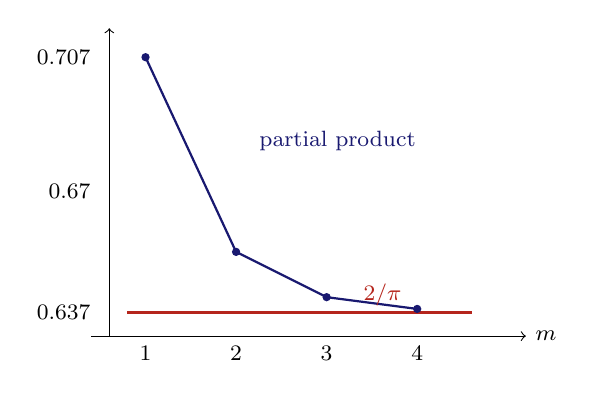
\begin{tikzpicture}[x=1.15cm,y=1.15cm,every node/.style={font=\footnotesize}]
  \draw[->,black] (0.4,0)--(5.2,0) node[right] {$m$};
  \draw[->,black] (0.6,0)--(0.6,3.4);
  \draw[BrickRed,thick] (0.8,0.26)--(4.6,0.26);
  \draw[MidnightBlue,thick] (1,3.08)--(2,0.93)--(3,0.43)--(4,0.30);
  \foreach \m/\y in {1/3.08,2/0.93,3/0.43,4/0.30} {
    \fill[MidnightBlue] (\m,\y) circle (1.5pt);
    \node[below] at (\m,0) {$\m$};
  }
  \node[anchor=east] at (0.5,0.26) {$0.637$};
  \node[anchor=east] at (0.5,1.60) {$0.67$};
  \node[anchor=east] at (0.5,3.08) {$0.707$};
  \node[BrickRed,anchor=west] at (3.3,0.45) {$2/\pi$};
  \node[MidnightBlue,anchor=west] at (2.15,2.15) {partial product};
\end{tikzpicture}
